\documentclass[conference]{IEEEtran}
\IEEEoverridecommandlockouts
% The preceding line is only needed to identify funding in the first footnote. If that is unneeded, please comment it out.
\usepackage{cite}
\usepackage{amsmath,amssymb,amsfonts}
\usepackage{algorithmic}
\usepackage{graphicx}
\usepackage{textcomp}
\usepackage{xcolor}
\usepackage[brazilian]{babel}
\usepackage[utf8]{inputenc}
\usepackage[T1]{fontenc}
\usepackage{listings}
\usepackage{color}
\usepackage{float}
\usepackage{multirow}
\usepackage{hyperref}

\definecolor{dkgreen}{rgb}{0,0.6,0}
\definecolor{gray}{rgb}{0.5,0.5,0.5}
\definecolor{mauve}{rgb}{0.58,0,0.82}

\lstset{frame=tb,
  language=Java,
  aboveskip=3mm,
  belowskip=3mm,
  showstringspaces=false,
  columns=flexible,
  basicstyle={\small\ttfamily},
  numbers=none,
  numberstyle=\tiny\color{gray},
  keywordstyle=\color{blue},
  commentstyle=\color{dkgreen},
  stringstyle=\color{mauve},
  breaklines=true,
  breakatwhitespace=true,
  tabsize=3
}
\lstset{language=Python}
\def\BibTeX{{\rm B\kern-.05em{\sc i\kern-.025em b}\kern-.08em
    T\kern-.1667em\lower.7ex\hbox{E}\kern-.125emX}}
\begin{document}

\title{Relatório da Atividade 1: \\ Logical Clock\\
}

\author{\IEEEauthorblockN{Isabelle Ferreira de Oliveira}
\IEEEauthorblockA{\textit{CES-27 - Engenharia da Computação 2020} \\
\textit{Instituto Tecnológico de Aeronáutica (ITA)}\\
São José dos Campos, Brasil \\
isabelle.ferreira3000@gmail.com}
}

\maketitle

\begin{abstract}
Esse relatório documenta a implementação da simulação de processos rodando e trocando seus relógios lógicos entre si (Logical Clock definido por Lamport). Esses relógios foram tanto escalares quanto vetoriais.
\end{abstract}

\begin{IEEEkeywords}
Relógio lógico, Relógio lógico escalar, Relógio lógico vetorial, algoritmo de Lamport
\end{IEEEkeywords}

\section{Implementação}

	\subsection{Tarefa 1: Relógio Lógico Escalar}
	
	Essa primeira etapa se tratou da implementação do método build\underline{\space}model() da classe DQNAgent de dqn\underline{\space}agent.py, script fornecido no código base do laboratório. Nesse método, era preciso construir uma rede em Keras de acordo com as especificações apresentadas na Tabela 3 do roteiro do laboratório \cite{roteiro}.
	
	Essa implementação foi feita de forma bastante análoga à maneira do laboratório 8 \cite{roteiro8}, ou seja, seguindo o apresentado no pseudo-código em Python a seguir.
	
\begin{lstlisting}
# Adds the first layer
model.add(layers.Dense(num_neurons,
	activation=activations.some_function,
	input_dim=state_size))

# Adds another layer (not first)
model.add(layers.Dense(num_neurons,
	activation=activations.some_function))
\end{lstlisting}

	Vale ressaltar que, para atender os critérios requisitados, some\underline{\space}function do pseudo-código acima se tratou de \textit{relu} para as duas primeiras camadas, e de \textit{linear} para terceira camada. Além disso, num\underline{\space}neurons foram 24, 24 e action\underline{\space}size para as primeira, segunda e terceira camada, respectivamente.

	Fora isso, bastou-se descomentar as linhas de criação de uma pilha linear de camadas, as linhas compilação do modelo e impressão do summary do modelo, apresentado futuramente na seção \ref{results} (Resultados e Conclusões), e a linha de retorno da função.

	\subsection{Tarefa 2: Relógio Lógico Vetorial}

	Já essa etapa se tratou da implementação do método act() também da classe DQNAgent de dqn\underline{\space}agent.py. Nesse método, era escolhido e retornado uma ação de acordo com a política $\epsilon$-greedy.
	
	Essa implementação foi feita de forma bastante análoga à maneira do laboratório 12 \cite{roteiro12}. Assim, gerou-se um número aleatório entre 0 e 1 e, caso esse valor aleatório seja menor que epsilon, então uma ação aleatória é escolhida; caso contrário, é escolhida a ação gulosa, através do retorno do índice do máximo elemento do array \textit{model.predict(state)[0]}.
		
	\subsection{Reward Engineering}
	
	Nesse momento, foi implementado o método reward\underline{\space}engineering\underline{\space}mountain\underline{\space}car() de utils.py, script também fornecido no código base do laboratório. Nesse método, eram calculadas e retornadas as recompensas intermediárias "artificias", chamadas reward engineering, a fim de tornar o treino mais rápido no ambiente do Mountain Car.
	
	Essa implementação foi feita conforme as equações apresentadas na seção 4.3 do roteiro do laboratório \cite{roteiro}, ou seja, assim como apresentado no pseudo-código em Python a seguir.
	
\begin{lstlisting}
reward = reward + (position - start) * (position - start) + velocity * velocity

aux = 0
if next_position >= 0.5:
    aux = 1

reward += 50 * aux
\end{lstlisting}

	Os valores de position, start, velocity e next\underline{\space}position também eram fornecidos no roteiro \cite{roteiro}, e bastava substituí-los no pseudo-código acima.

	\subsection{Treinamento usando DQN}
	
	Bastava treinar o modelo implementado, executando o script train\underline{\space}dqn.py, também do código base, e observar os resultados e os gráficos obtidos.

	\subsection{Avaliação da Política}
	
	Bastava aplicar o modelo implementado no ambiente do Mountain Car, executando o script evaluate\underline{\space}dqn.py, também do código base, e observar a simulação, os resultados e os gráficos obtidos.

\section{Resultados e Conclusões} \label{results}

	O summary do modelo implementado em make\underline{\space}model() foi apresentado na Figura \ref{summary}, e condiz com os requisitos pedidos na Tabela 3 do roteiro do laboratório \cite{roteiro}. 

\begin{figure}[htbp]
\centering
\centerline{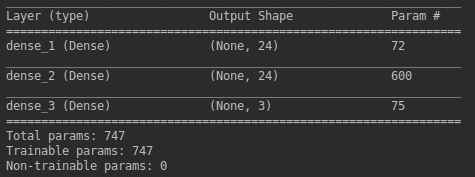
\includegraphics[scale=0.5]{imagens/summary.png}}
\caption{Sumário do modelo implementado em Keras.}.
\label{summary}
\end{figure}

	Já a Figura \ref{train/15} representa as recompensas acumulativas advindas do treinamento do modelo em 300 episódios. Esse resultado dependem diretamente da correta implementação e funcionamento dos métodos make\underline{\space}model() e act().
	
	Pode-se dizer que esse gráfico condiz com o esperado, uma vez que é possível notar inicialmente recompensas pequenas para os primeiros episódios e, mais ou menos a partir do episódio 80, tornou-se frequente recompensas com valores elevados, chegando a valores próximos de 40, indicando um aprendizado significantemente correto.

\begin{figure}[htbp]
\centering
\centerline{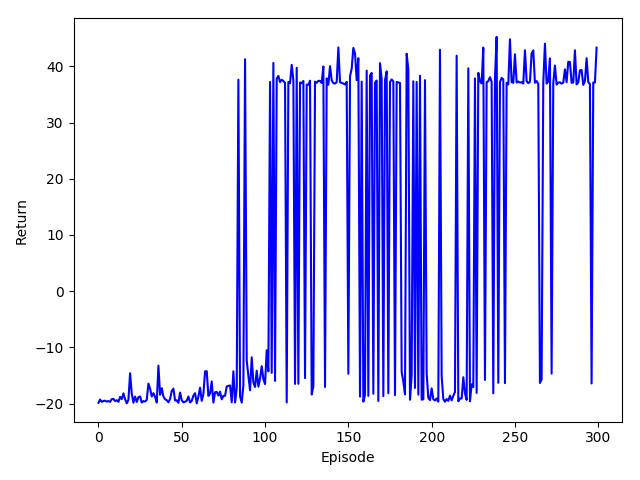
\includegraphics[scale=0.3]{imagens/train/15.png}}
\caption{Recompensa acumulativa com o passar dos episódios, no treinamento do modelo para 300 episódios.}.
\label{train/15}
\end{figure} 

	Já a aplicação do modelo implementado no ambiente do Mountain Car gerou as Figuras de \ref{dqn_evaluation} a \ref{agent_decision}.
	
	A partir da Figura \ref{dqn_evaluation}, pode-se concluir que a implementação e treino chegaram em resultados satisfatórios, uma vez que grande parte das recompensas acumuladas foi alta, próximas de 40, chegando no final de 30 episódios a uma média de 27.8, conforme apresentado na Figura \ref{evaluate_dqn_result}.
	
\begin{figure}[htbp]
\centering
\centerline{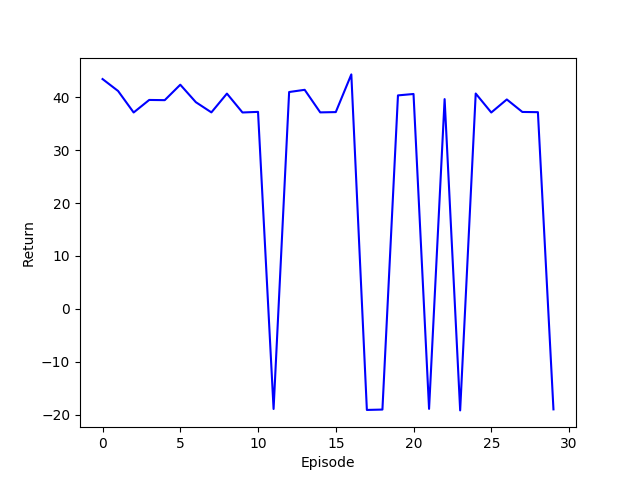
\includegraphics[scale=0.5]{imagens/dqn_evaluation.png}}
\caption{Representação em cores da tabela de action-value calculada, para algoritmo de Sarsa.}.
\label{dqn_evaluation}
\end{figure}

\begin{figure}[htbp]
\centering
\centerline{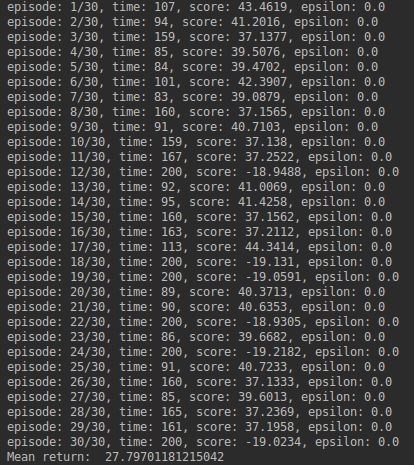
\includegraphics[scale=0.4]{imagens/evaluate_dqn_result.png}}
\caption{Recompensa acumulada em função das iterações, para algoritmo de Sarsa.}.
\label{evaluate_dqn_result}
\end{figure}
	
	Por fim, acerca da Figura \ref{agent_decision}, pode-se observar que:
	
\begin{itemize}

\item Para velocidades para direita, quase unanimamente a decisão do carro é continuar para direita. Exclui-se disso as situações de posição muito à esquerda e velocidades altas, na qual é decidido fazer nada, e de velocidades para direita muito baixas, na qual pouquíssimas vezes o carro decide ir para esquerda, talvez já se enquadrando nas intenções descritas no próximo item.

\item Para velocidades para esquerda, as decisões do carro diferem bastante da posição na qual ele se encontra. Para posições mais a esquerda, o carro decide continuar indo para esquerda, talvez para pegar impulso da subida e, quando por fim chegar em posições mais a esquerda (consequentemente mais altas) possíveis, decidir ir com velocidade para direita. Já para posições relativamente próximas da posição objetivo, aparecem também decisões de não fazer nada, indicando que o carro irá mais para esquerda e cairá na situação anteriormente descrita, na qual ele decidirá continuar indo para esquerda e pegará o impulso da elevação.

\end{itemize}

\begin{figure}[htbp]
\centering
\centerline{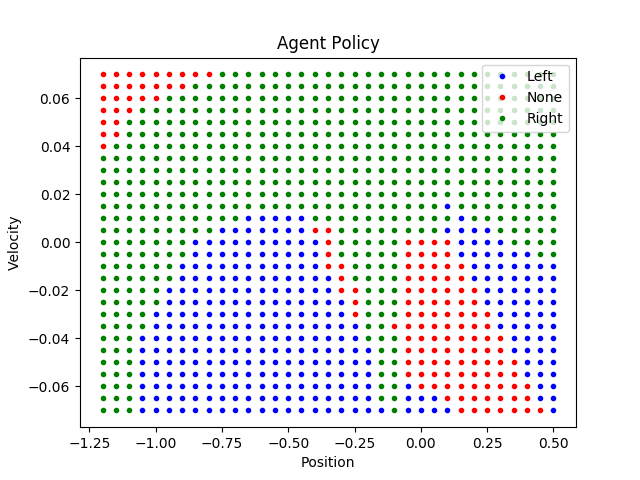
\includegraphics[scale=0.5]{imagens/agent_decision.png}}
\caption{Representação em cores da tabela de greedy-policy calculada, para algoritmo de Sarsa.}.
\label{agent_decision}
\end{figure} 

Como as decisões aprendidas e tomadas pelo carro fizeram sentido e puderam ser interpretadas satisfatoriamente, pode-se dizer que a proposta do laboratório foi corretamente implementada e se mostrou satisfatória em resolver o problema proposto.
	
\begin{thebibliography}{00}
\bibitem{roteiro} M. Maximo, ``Roteiro: Laboratório 12 - Deep Q-Learning''. Instituto Tecnológico de Aeronáutica, Departamento de Computação. CT-213, 2019.

\bibitem{roteiro8} M. Maximo, ``Roteiro: Laboratório 8 - Imitation Learning com Keras''. Instituto Tecnológico de Aeronáutica, Departamento de Computação. CT-213, 2019.

\bibitem{roteiro12} M. Maximo, ``Roteiro: Laboratório 12 - Aprendizado por Reforço Livre de Modelo''. Instituto Tecnológico de Aeronáutica, Departamento de Computação. CT-213, 2019.

\end{thebibliography}

\end{document}
